\section{2020 年 10 月 31 日答疑记录}


\begin{example}\label{exa:201115-1040}
    求函数 $f(t)= \dfrac{t^2-4t+1}t$ ($t>0$) 的最小值和对应的 $t$ 的值.
\end{example}
\begin{solution}
    因为 $t>0$, 所以由均值不等式, 
    \[f(t)= \frac{t^2-4t+1}t= t+\frac1t-4
        \geqslant 2\sqrt{t\cdot\frac1t}-4= -2,\]
    ``$=$'' 成立当且仅当 $t=\dfrac1t$ 即 $t=1$. 以上表明 $f_{\min}=-2$, 且对应的 $t=1$.
\end{solution}
\begin{remark}
    (1) 求值域的一般方法是讨论单调性, 但对特殊的分式函数, 则一般先考虑用均值不等式. 例~\ref{exa:201115-1040} 中还可以推导如下:
    \[f(t)= \frac{t^2-4t+1}t= \frac{t^2+1-4t}t
        \geqslant \frac{2\sqrt{t^2\cdot1}-4t}t= -2.\]
    
    (2) 用均值不等式时, 必须考虑等号成立的条件. 如果例~\ref{exa:201115-1040} 中 $t\geqslant 3$, 那么等号就不能成立, 只能写 $f(t)>-2$, 即不能得到 $f_{\min}=-2$ 的结论. 此时的解法参可借用例~\ref{exa:201115-1045} 中的单调性结论.
\end{remark}

\begin{example}\label{exa:201115-1045}
    函数 $f(x)= x+\dfrac1x$ ($x\neq 0$) 是奇函数还是偶函数? 写出其单调区间.
\end{example}
\begin{solution}
    因为 
    \[f(-x)= (-x)+\frac1{-x}= -\biggl(x+\frac1x\biggr)= -f(x),\]
    所以 $f(x)$ 是奇函数.
    
    当 $x$ 是充分小的正数时, $f(x)\approx \dfrac1x$; 当 $x$ 是充分大的正数时, $f(x)\approx x$. 再结合
    \[f\biggl(\frac14\biggr)= f(4)= \frac{17}4,\ 
      f\biggl(\frac13\biggr)= f(3)= \frac{10}3,\ 
      f\biggl(\frac12\biggr)= f(2)= \frac{5}2,\ 
      f(1)= 2,\]
    可以描点作图如下 (第三象限的图形与第一象限的图形关于原点对称):
    \begin{center}
        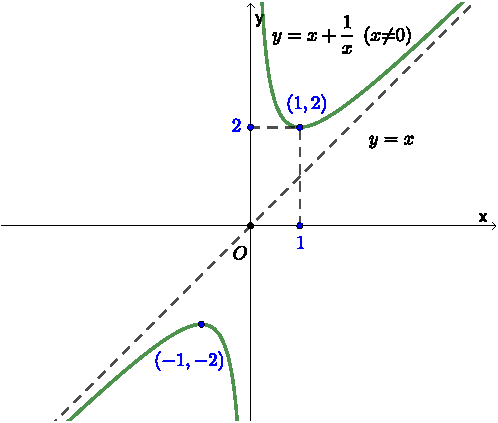
\includegraphics[scale=1]{2020-1115-1100-crop}
    \end{center}
    由图可以看出 $f(x)$ 的单调递增区间为 $(-\infty,-1]$ 和 $[1,+\infty)$, 单调递减区间为 $(-1,0)$ 和 $(0,1)$.
\end{solution}

例~\ref{exa:201115-1045} 中的函数 $f(x)= x+\dfrac1x$ ($x\neq 0$) 一般形象地称为 ``对勾函数'', 第一象限图形的最低点 $(1,2)$ 可由均值不等式得到. $f(x)$ 的图形有两条渐近线: $y=x$ 和 $x=0$ (即 $y$~轴), 符合双曲线的特点 (有两条渐近线). 观察 $f(x)$ 的图形可知, 若 $x\geqslant 3$, 则 $f(x)\geqslant f(3)$, 即此时 $f_{\min}=f(3)$. 类似地, 若 $x\geqslant \dfrac12$, 则 $f_{\min}=f(1)$. 

一般地, $f(x)= x+\dfrac{k}x$ ($k>0$, $x\neq 0$) 均可称为 ``对勾函数''. 由与前面类似的分析可得, $f(x)$ 是奇函数, 有两条渐近线 $y=x$ 和 $x=0$, 第一象限图形的最低点为 $(\sqrt{k},2\sqrt{k})$, 单调递增区间为 $(-\infty,-\sqrt{k}]$ 和 $[\sqrt{k},+\infty)$, 单调递减区间为 $(-\sqrt{k},0)$ 和 $(0,\sqrt{k})$.

\begin{example}\label{exa:201115-1130}
    若函数 $f(x)= \begin{cases}
        x-1, & x\leqslant 1,\\
        x^2+a, & x>1
    \end{cases}$ 在 $\realnum$ 上单调递增, 求实数 $a$ 的取值范围.
\end{example}
\begin{solution}
    由题意,
    \[1-1\leqslant 1^2+a\ \text{即}\ a\geqslant -1,\]
    所以 $a\in[-1,+\infty)$.
\end{solution}

解分段函数单调性问题时, 只需每段函数均单调, 且分段点处的函数值满足题中单调性. 具体来说,
\begin{align*}
    &f(x)= \begin{cases}
            g(x), & x\leqslant a,\\
            h(x), & x>a
        \end{cases}\ \text{在 $\realnum$ 上单调递增}\\
    \Leftrightarrow{}& \left\{\!\!\begin{array}{l}
        \text{$g(x)$ 在 $(-\infty,a]$ 上, $h(x)$ 在 $(a,+\infty)$ 上均单调递增},\\
        g(a)\leqslant h(a)
        \end{array}\right.\\
    &f(x)= \begin{cases}
            g(x), & x\leqslant a,\\
            h(x), & x>a
        \end{cases}\ \text{在 $\realnum$ 上单调递减}\\
    \Leftrightarrow{}& \left\{\!\!\begin{array}{l}
        \text{$g(x)$ 在 $(-\infty,a]$ 上, $h(x)$ 在 $(a,+\infty)$ 上均单调递减},\\
        g(a)\geqslant h(a)
        \end{array}\right.\\
\end{align*}
建议结合如下函数草图记忆上述结论:
\begin{center}
    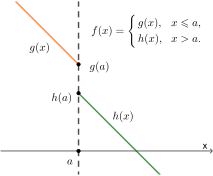
\includegraphics[scale=1]{2020-1115-1130-1-crop}\qquad
    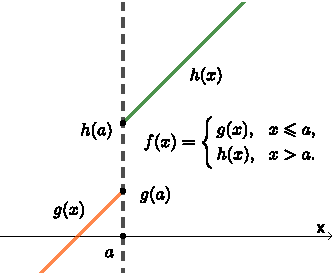
\includegraphics[scale=1]{2020-1115-1130-2-crop}
\end{center}

如果例~\ref{exa:201115-1130} 改为 ``函数 $f(x)= \begin{cases}
    x-1, & x\leqslant 1,\\
    x^2+2ax, & x>1
\end{cases}$ 在 $\realnum$ 上单调递增'', 则应限制
\[\begin{cases}
    -a\leqslant 1 & (\text{二次函数对称轴在定义域左侧}),\\
    1-1\leqslant 1^2+ 2a\cdot1 & (\text{分段点处的函数值递增}).
    \end{cases}\]


\begin{example}\label{exa:201115-1140}
    设定义在 $(-1,1)$ 上的奇函数 $f(x)$ 是增函数, 解关于 $a$ 的不等式 
    \[f(a)+f(2a-1)<0.\]
\end{example}
\begin{solution}
    因为 $f(x)$ 是奇函数, 所以已知不等式化为
    \[f(a)<-f(2a-1)= f(1-2a).\]
    再结合 $f(x)$ 在 $(-1,1)$ 上是增函数可知
    \[\left\{\!\!\begin{array}{l}
        -1<a<1,\ -1<1-2a<1\\
        a<1-2a,
        \end{array}\right.\ \text{解得}\quad a\in\biggl(0,\frac13\biggr).\]
\end{solution}
\begin{remark}
    例~\ref{exa:201115-1140} 中的不等式 $f(a)+f(2a-1)<0$ 可以称为 ``抽象不等式'' (因为没有具体的表达式), 这类不等式一般先化为 ``$f(a)<f(b)$'' 的形式, 再利用函数的单调性去掉 ``$f$'' 而转化为具体不等式 ``$a<b$'' 或 ``$a>b$''.
\end{remark}


\begin{example}
    求函数 $f(x)=\dfrac{2x+1}{x-1}$, $x\in[-8,-4)$ 的值域.
\end{example}
\begin{solution}
    先把已知函数变形 (一次式除以一次式的常用变形方法),
    \[f(x)=\frac{2x+1}{x-1}= \frac{2(x-1)+3}{x-1}= 2+ \frac3{x-1},\]
    再利用函数图形平移 (上加下减, 左加右减) 利用 $y=\dfrac3x$ 的图形可知 $f(x)$ 的图形如下:
    \begin{center}
        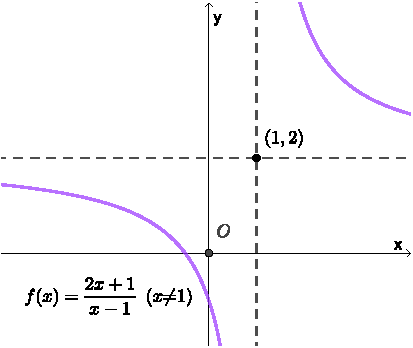
\includegraphics[scale=1]{2020-1115-1210-crop}
    \end{center}
    所以 $f(x)$ 在 $[-8,-4)$ 上单调递减, 值域为 $(f(-4),f(-8)]= \biggl(\dfrac75,\dfrac53\biggr]$ (即最大值为 $\dfrac53$, 无最小值).
\end{solution}

\begin{example}\label{exa:201115-1210}
    已知 $f(x)= ax^7-bx^5+cx^3+2$, 且 $f(-5)=m$, 求 $f(-5)+f(5)$ 的值.
\end{example}
\begin{solution}
    直接代入知,
    \begin{align*}
    f(-5)+f(5)
      ={}& [a\cdot (-5)^7- b\cdot (-5)^5+ c\cdot (-5)^3+2] \\
         & + [a\cdot 5^7- b\cdot 5^5+c\cdot 5^3+2]\\
      ={}& 4.\end{align*}
\end{solution}

例~\ref{exa:201115-1210} 中的 ``$f(-5)=m$'' 是多余的条件. 如果注意到 $g(x)=ax^7-bx^5+cx^3$ 是奇函数, 则可以简洁地得到更一般地结论:
\[f(-x)+f(x)= [g(-x)+g(x)]+2\cdot 2= 4.\]